\subsection{EPR Paradox}
	Einstein-Podolski-Rosen (35)
	
	Grundannahme: Es existiert keinen ``fundamentaler'' Zufall.
	
	Zufall der Quantenmechanik ist irgendwie statistisch begründet.
	
	Die Quantenmechanik ist daher nicht vollständig. Verborgene Variablen.
	
	Version von Bohm: BILD
%	\begin{figure}
%		\begin{center}
%			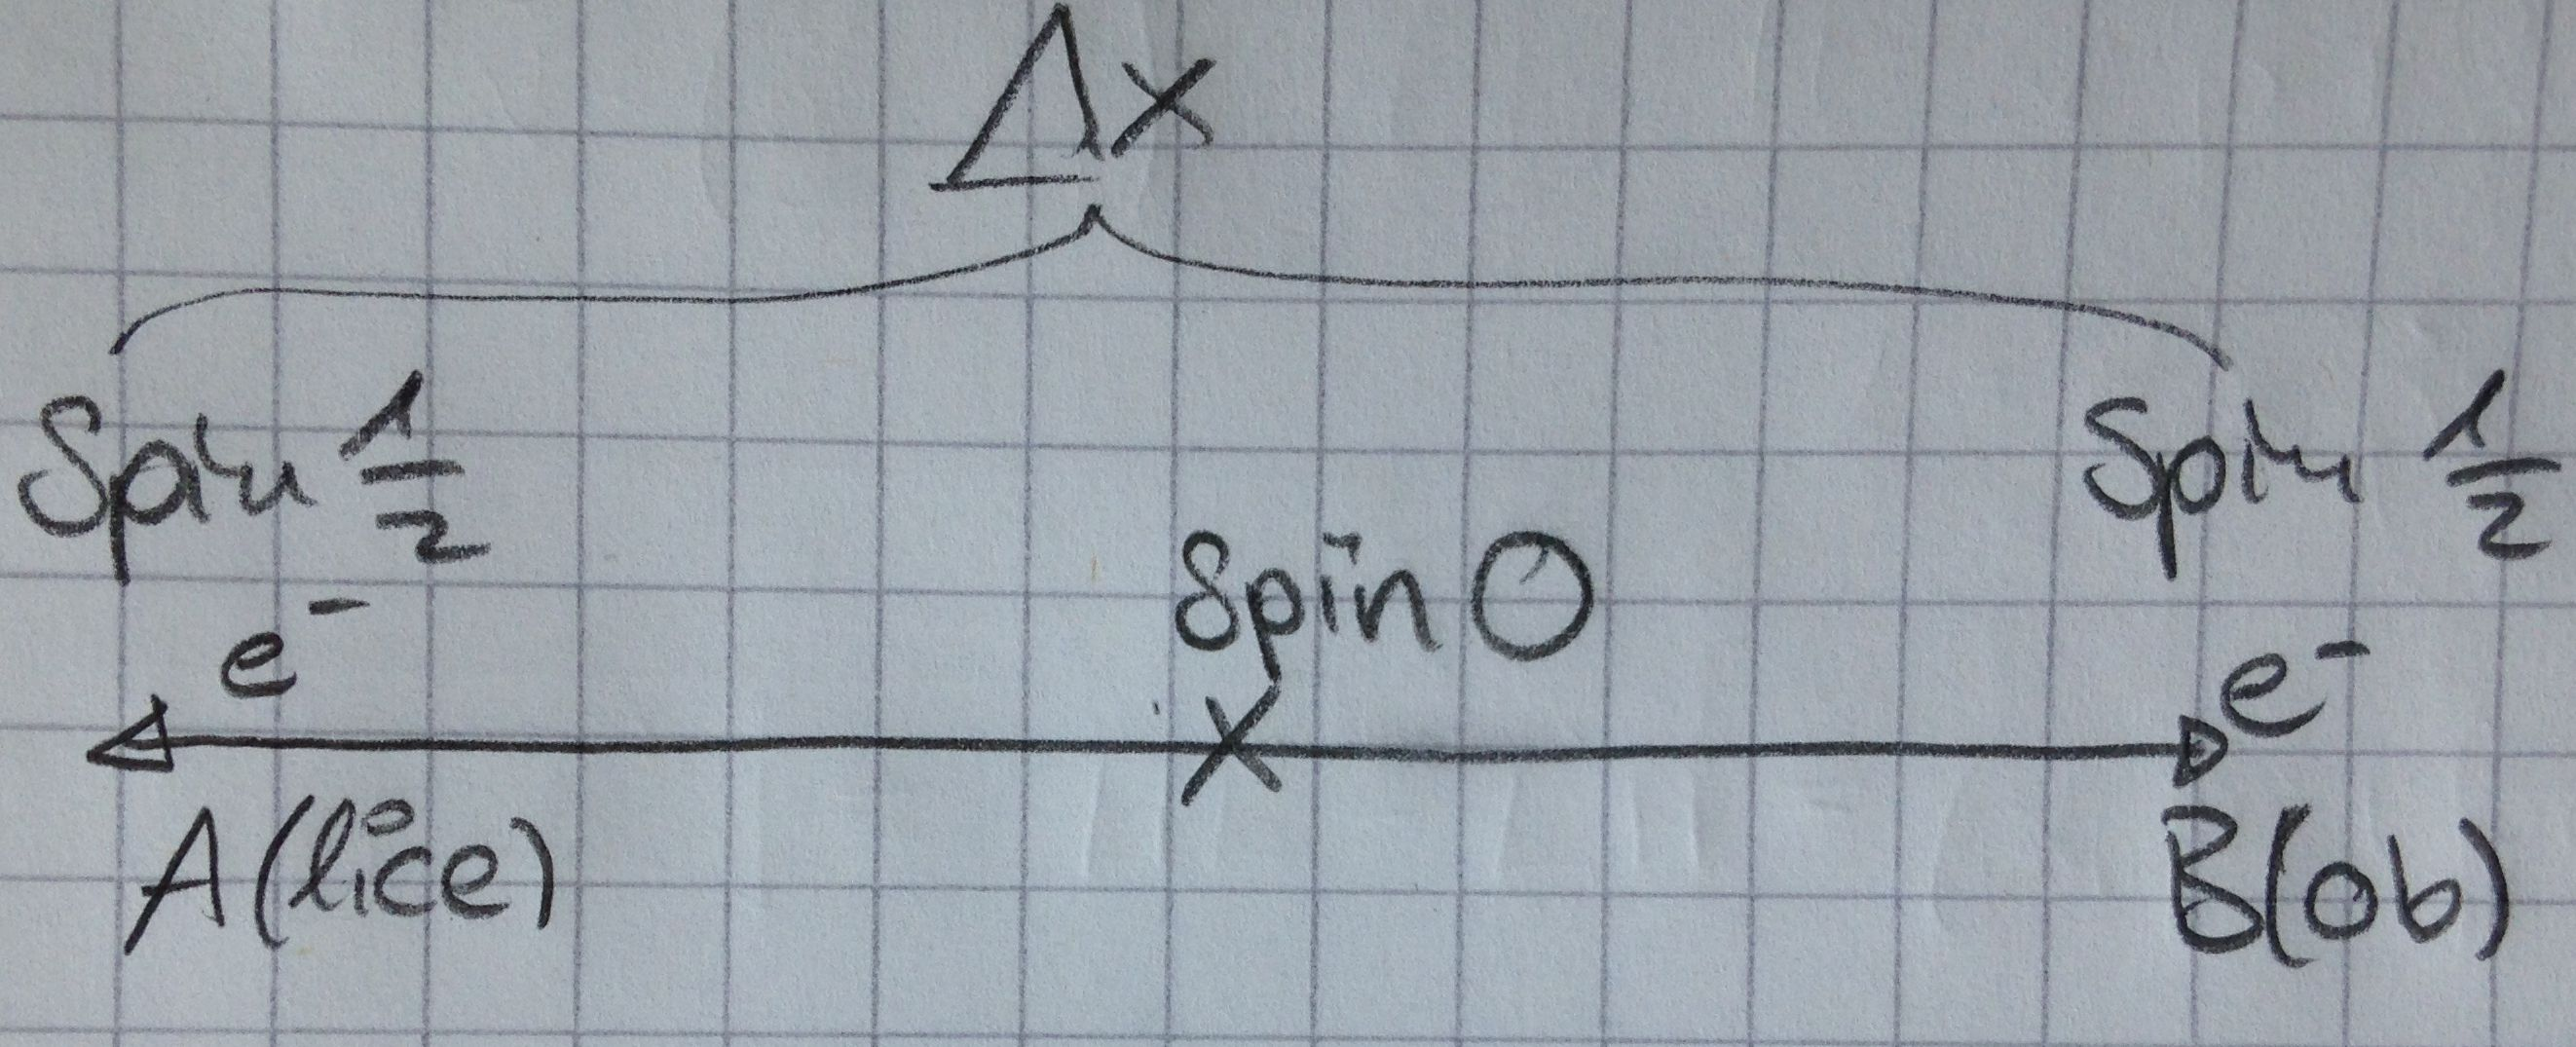
\includegraphics[content...]{EPR_Paradox}
%		\end{center}
%	\end{figure}

	Drehimpulserhaltung, Singulettzustand: $S_z^{(A)} = -S_z^{(B)}$
		\begin{align*} 
			S_{z}^{(A)} &= + \frac{\hbar}{2} &
			&\Leftrightarrow &S_z^{(B)} &= -\frac{\hbar}{2} \\
			S_z^{(A)} &= -\frac{\hbar}{2}& &\Leftrightarrow &S_z^{(B)} &= + \frac{\hbar}{2} \\
			S_x^{(A)} &= + \frac{\hbar}{2}& &\Leftrightarrow &S_x^{(B)} &= - \frac{\hbar}{2} 
		\end{align*}
	Zur Zeit $t_A$ werde in $A ~ S_z^{(A)} = + \frac{\hbar}{2}$ gemessen
	
	$\Rightarrow$ Zur Zeit $t_B = t_A + \Delta t$ wird $B$ mit Wahrscheinlichkeit 1 $S_z^{(B)} = -\frac{\hbar}{2}$ messen.
	
	(``verschränkter'' Zustand)
